\chapter{CNNs for computer vision}
\label{image-ann}

A paper Visualizing and Understanding Convolutional Networks by Matthew D. Zeiler and Robert Fergus \cite{zf-net} started with two sentences: \textit{Large Convolutional Network models have recently demonstrated impressive classification performance on the ImageNet benchmark. However there is no clear understanding of why they perform so well, or how they might be improved.}

I tried to disperse such clouds a bit in the previous chapter, but now I would like to focus on another undertone connected with those statements. On their applications in the computer vision.

Almost everything mentioned in chapter \ref{cnn} was already tied to the computer vision. The following text will briefly describe the field of computer vision itself and then introduce few tasks in that field connected with the topic of the thesis. In each task, few \zk{CNN} models will be mentioned. This text structure was chosen also to depict the models evolution concluding in the one selected for the practical part of this thesis - an implementation into GRASS GIS.

% different sizes

\section{Understanding computer vision}
\label{computer-vision}

When you see a group photo, you can easily count the number of people in the photo, you can say whether they are smiling or not, whether they are happy, sad, angry, you can even guess whether they are one family, a bunch of friends, colleagues or just random people passing by. You can do all of that in a fraction of a second without any effort. The computer vision is supposed to be a computer-aided version of this human cognition. Or in a fancier way, from \cite{opencv}: \textit{Computer vision is the transformation of data from a still or video camera into either a decision or a new representation.} The new representation might be for instance a colour shift, the decision an answer on a question like \textit{Is there any football field in the picture?}

However, the problem is that the claim that it is easy for humans does not mean that it is easy also for computers. As is generally known and was indicated in chapter \ref{understanding-cnn}, the human brain is an extremely complex tool. The other thing is that a computer receives a visual impulse (image) in other way as is illustrated in figure \ref{fig:mirror}. Where human sees a side mirror, a computer sees a grid of numbers. And this grid may be completely different when the daytime, viewpoint, brightness, background or scale changes.

\begin{figure}[H]
   \centering
	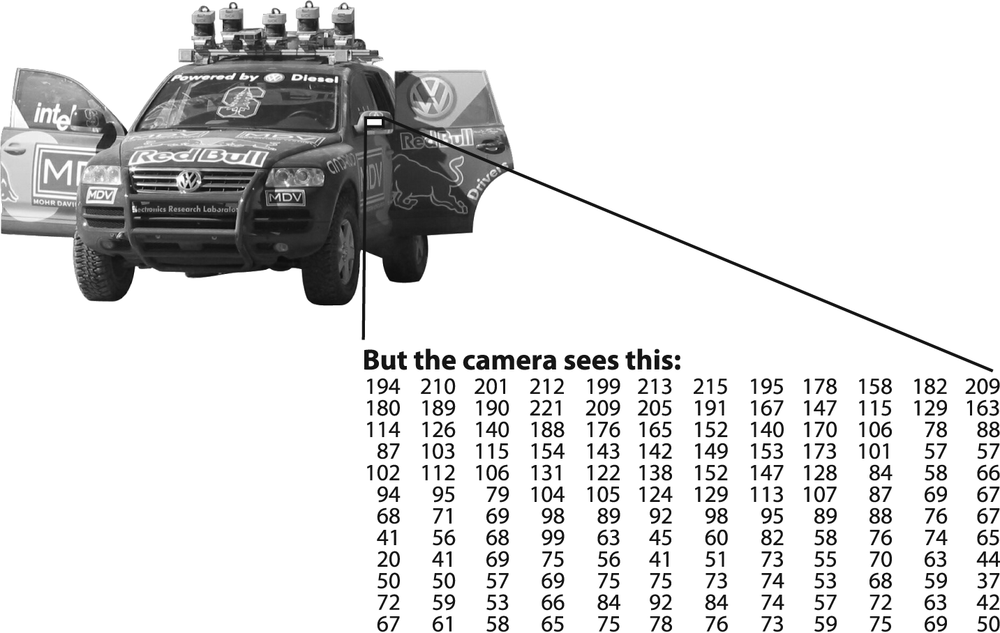
\includegraphics[width=.8\linewidth]{./pictures/comp-vision.png}
	\caption[Human and computer cognition]{The difference between human and computer cognition, source: \cite{opencv}}
      \label{fig:mirror}
\end{figure}

The task may be something like \textit{Is there any side mirror in the picture?} This kind of tasks can be seen in the field of computer vision daily and can be extremely difficult to solve in the computer way. Although the input may include some metadata, it still has to be solved in a strict mathematical way. And because our goal is to make our computer vision system \textit{perceive like a human}, it looks like the right place for \zk{CNN}s.

Although we will focus only on classification and connected tasks like detection and segmentation, there are many more applications of the computer vision. To name a few: Autonomous cars, face recognition, fingerprint recognition, motion capture, biometrics and remote sensing.

To get a better view into the field of computer vision, it is recommended to read a richer source like \cite{comp-vision} and \cite{opencv} to get some practice.

\section{Classification}
\label{classification}

\section{Classification with localization}
\label{classification-localization}

\section{Object detection}
\label{object-detection}

\subsection{R-CNN}
\label{r-cnn}

% R-CNN, Fast, Faster
% Single-Shot MultiBox Detector (SSD) You Only Look Once (YOLO)

\section{Semantic segmentation}
\label{semantic-segmentation}

% CNN

\section{Instance segmentation}
\label{instance-segmentation}

% Mask R-CNN

% \section{Content-based Image Retrieval}